\documentclass[a4paper]{article}

\usepackage[czech]{babel} %https://github.com/michal-h21/biblatex-iso690
\usepackage[
   backend=biber      % if we want unicode 
  ,style=iso-numeric % or iso-numeric for numeric citation method          
  ,babel=other        % to support multiple languages in bibliography
  ,sortlocale=cs_CZ   % locale of main language, it is for sorting
  ,bibencoding=UTF8   % this is necessary only if bibliography file is in different encoding than main document
]{biblatex}

\usepackage[utf8]{inputenc}
\usepackage{fancyhdr}
\usepackage{amsmath}
\usepackage{amssymb}
\usepackage[left=2cm,right=2cm,top=2.5cm,bottom=2.5cm]{geometry}
\usepackage{graphicx}
\usepackage{pdfpages}
\usepackage{url}

\usepackage{siunitx}
\sisetup{locale = DE}  %, separate-uncertainty = true    kdybych chtel +/-

\usepackage{float}
\newfloat{graph}{htbp}{grp}
\floatname{graph}{Graf}
\newfloat{tabulka}{htbp}{tbl}
\floatname{tabulka}{Tabulka}

\renewcommand{\thefootnote}{\roman{footnote}}

\pagestyle{fancy}
\lhead{Praktikum III - (27) Kerrův jev v pevné látce}
\rhead{Vladislav Wohlrath}
\author{Vladislav Wohlrath}

\bibliography{source}

\begin{document}

\begin{titlepage}
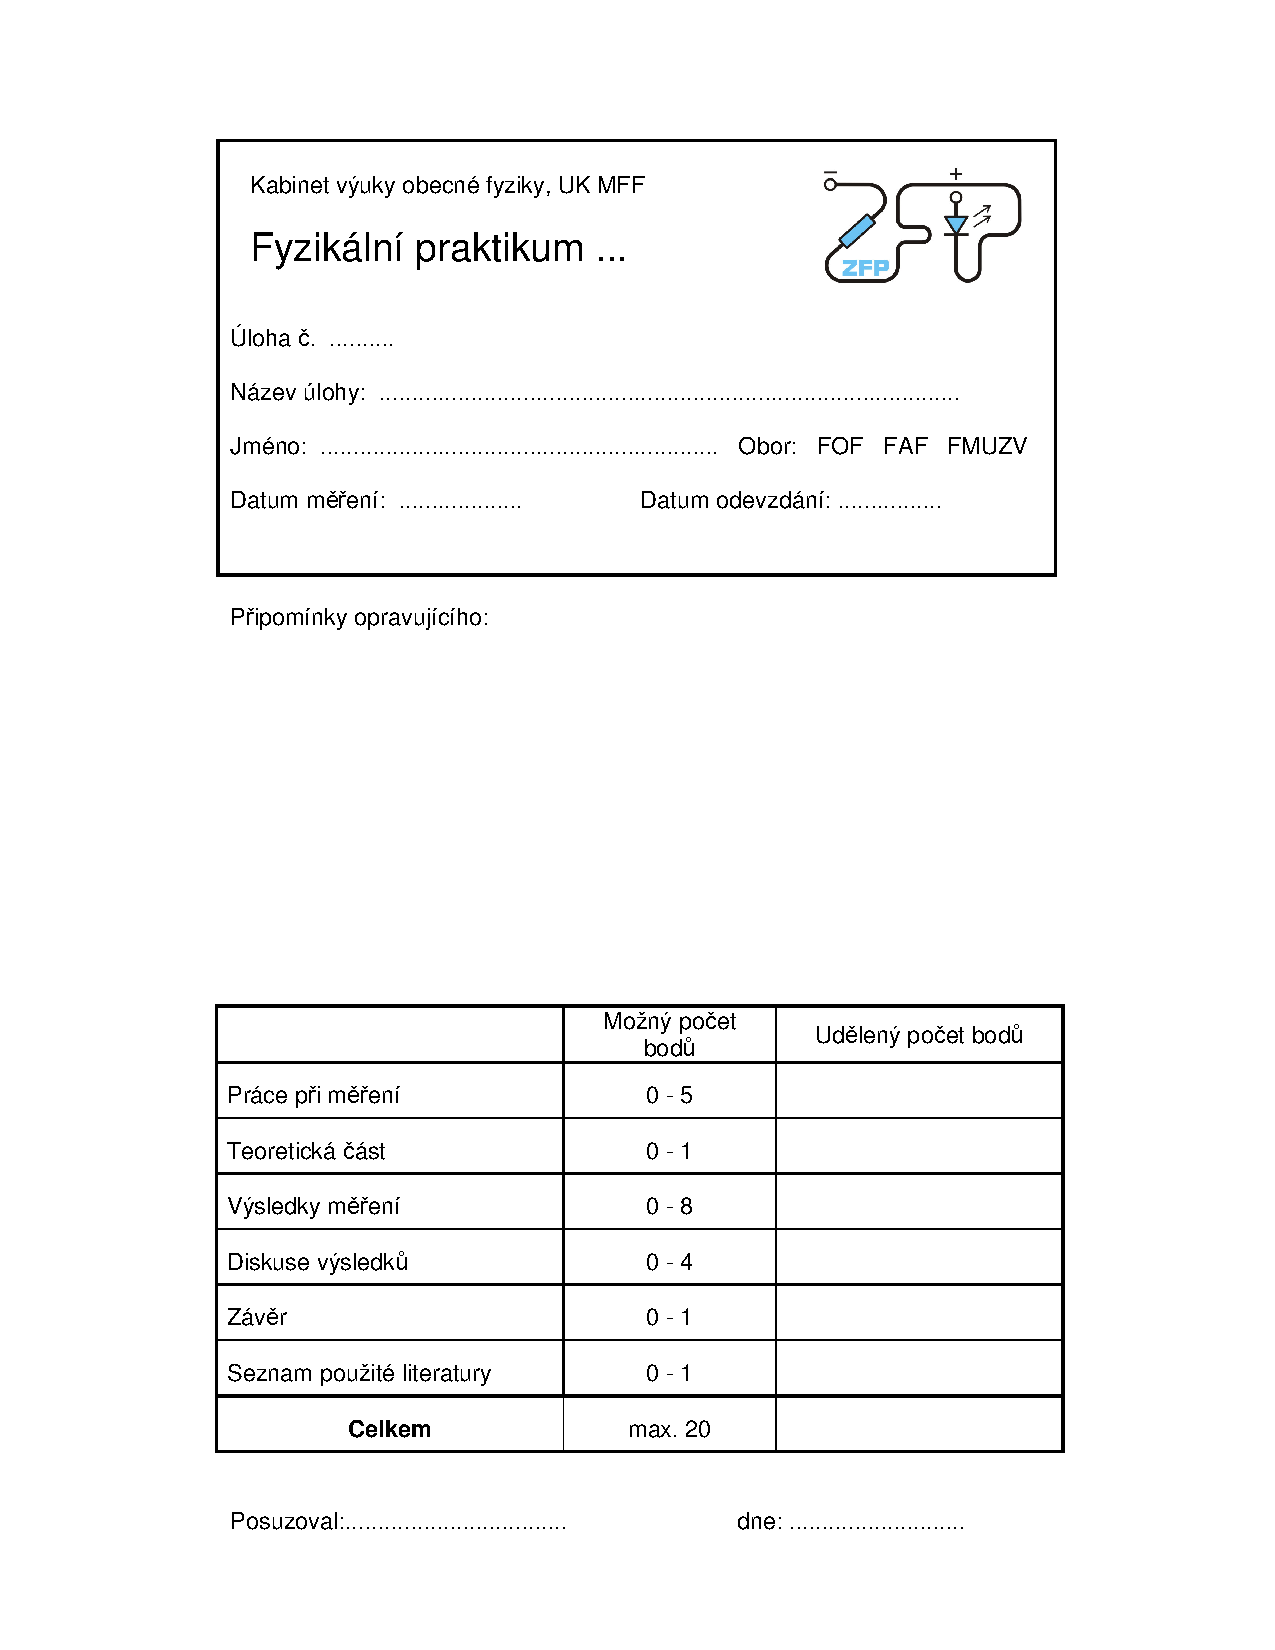
\includepdf[pages={1}]{./graficos/titlelist.pdf}
\end{titlepage}

\section*{Pracovní úkoly}
\begin{enumerate}
\item Sestavte aparaturu pro sledování příčného elektrooptického jevu v pevném vzorku. Laser umístěte tak, aby byl zdroj světla polarizován kolmo k vodorovné rovině. (Předem najděte směr snadného průchodu polarizátorů používaných v aparatuře).
\item Změřte závislost intenzity světla dopadající na detektor na napětí přiloženém na elektrody vzorku. Zpracujte graficky, určete půlvlnné napětí.
\item Ze směrnice závislosti fázového posunu mezi řádným a mimořádným paprskem na čtverci přiloženého napětí určete Kerrovu konstantu vzorku.
\end{enumerate}

%Teoretická část
\section*{Teoretická část}
Pokud PLZT vzorek vložíme do elektrostatického pole, stane se dvojlomným.
Pokud na vzorek budeme působit elektrickým polem o intenzitě $E$ a délku vzorku (vzdálenost, kterou v ní urazí světlo) označíme $l$, bude fázový posuv mezi oběma složkami vlny \cite{zfp}
\begin{equation}
\Delta = 2\pi \cdot K \cdot l \cdot E^2 \,,
\end{equation}
kde $K$ je Kerrova konstanta vzorku.

Elektrickou intenzitu můžeme vyjádřit pomocí přiloženého napětí $U$ a vzdálenosti elektrod $d$
\begin{equation}
E=\frac{U}{d} \,.
\end{equation}

Experiment uspořádáme podle návodu v \cite{zfp}. Polarizátory zkřížíme a vzorek umístíme tak, aby směr elektrického pole svíral s rovinou polarizace dopadajícího světla úhel \SI{45}{\degree}. Pro intenzitu světla za analyzátorem pak platí \cite{zfp}
\begin{equation}
I=I_0 \sin^2 \frac{\Delta}{2} \,,
\end{equation}
kde $I_0$ je intenzita v případě, že na vzorek přiložíme nulové napětí a směry průchodu světla polarizátorem a analyzátorem jsou shodné.

Dosazením za $\Delta$ dostáváme
\begin{equation}
I=I_0 \sin^2 \frac{\pi \cdot K \cdot  l \cdot E^2}{d^2}
\end{equation}
a po úpravě
\begin{equation} \label{e:fit}
\arcsin \sqrt{\frac{I}{I_0}} = K \cdot \frac{\pi l}{d^2} U^2 \,.
\end{equation}

Ze směrnice této závislosti určíme Kerrovu konstantu.

V případě $\Delta = \pi$, tedy rozdíl v optických drahách je roven $\lambda/2$, se vzorek chová jako půlvlnná destička a vycházející vlna je lineárně polarizovaná v rovině kolmé na původní rovinu polarizace, tedy ve směru snadného průchodu analyzátorem. V takovém případě naměříme maximum intenzity a hodnotu přiloženého napětí nazýváme půlvlnné napětí.

%Podmínky a měřící přístroje
\section*{Podmínky a použité přístroje}

%Výsledky měření
\section*{Výsledky měření}
Použili jsme červený laser.
Rozměry vzorku byly:
\begin{equation*}
l=\SI{1.5}{\mm} \qquad \qquad d=\SI{1.4}{\mm}
\end{equation*}

Směry snadného průchodu světla obou polarizátorů jsme určili metodou popsanou v \cite{zfp}.

Závislost $I$ na $U$ jsme změřili dvakrát, poprvé s časovými intervaly mezi změnami napětí \SI{1}{\minute}, podruhé s intervaly \SI{2}{\minute} a jemnějším měřením okolo půlvlnného napětí.

Časový průběh intenzity v obou měřeních je zaznamenán v grafech \ref{g:1} a \ref{g:2}. Časová osa nicméně neodpovídá skutečnému času, měření jsme vždy před nastavením napětí zastavili, a poté opět spustili. Proto se v grafech objevují nespojitosti. Oba grafy tedy slouží především ke sledování odezvy vzorku. Při studiu těchto grafů je také důležité mít na paměti, že vodorovná osa neodpovídá napětí, protože měřené hodnoty napětí nejsou ekvidistálně rozloženy.

\begin{graph}[htbp] 
\centering
% GNUPLOT: LaTeX picture with Postscript
\begingroup
  \makeatletter
  \providecommand\color[2][]{%
    \GenericError{(gnuplot) \space\space\space\@spaces}{%
      Package color not loaded in conjunction with
      terminal option `colourtext'%
    }{See the gnuplot documentation for explanation.%
    }{Either use 'blacktext' in gnuplot or load the package
      color.sty in LaTeX.}%
    \renewcommand\color[2][]{}%
  }%
  \providecommand\includegraphics[2][]{%
    \GenericError{(gnuplot) \space\space\space\@spaces}{%
      Package graphicx or graphics not loaded%
    }{See the gnuplot documentation for explanation.%
    }{The gnuplot epslatex terminal needs graphicx.sty or graphics.sty.}%
    \renewcommand\includegraphics[2][]{}%
  }%
  \providecommand\rotatebox[2]{#2}%
  \@ifundefined{ifGPcolor}{%
    \newif\ifGPcolor
    \GPcolortrue
  }{}%
  \@ifundefined{ifGPblacktext}{%
    \newif\ifGPblacktext
    \GPblacktextfalse
  }{}%
  % define a \g@addto@macro without @ in the name:
  \let\gplgaddtomacro\g@addto@macro
  % define empty templates for all commands taking text:
  \gdef\gplbacktext{}%
  \gdef\gplfronttext{}%
  \makeatother
  \ifGPblacktext
    % no textcolor at all
    \def\colorrgb#1{}%
    \def\colorgray#1{}%
  \else
    % gray or color?
    \ifGPcolor
      \def\colorrgb#1{\color[rgb]{#1}}%
      \def\colorgray#1{\color[gray]{#1}}%
      \expandafter\def\csname LTw\endcsname{\color{white}}%
      \expandafter\def\csname LTb\endcsname{\color{black}}%
      \expandafter\def\csname LTa\endcsname{\color{black}}%
      \expandafter\def\csname LT0\endcsname{\color[rgb]{1,0,0}}%
      \expandafter\def\csname LT1\endcsname{\color[rgb]{0,1,0}}%
      \expandafter\def\csname LT2\endcsname{\color[rgb]{0,0,1}}%
      \expandafter\def\csname LT3\endcsname{\color[rgb]{1,0,1}}%
      \expandafter\def\csname LT4\endcsname{\color[rgb]{0,1,1}}%
      \expandafter\def\csname LT5\endcsname{\color[rgb]{1,1,0}}%
      \expandafter\def\csname LT6\endcsname{\color[rgb]{0,0,0}}%
      \expandafter\def\csname LT7\endcsname{\color[rgb]{1,0.3,0}}%
      \expandafter\def\csname LT8\endcsname{\color[rgb]{0.5,0.5,0.5}}%
    \else
      % gray
      \def\colorrgb#1{\color{black}}%
      \def\colorgray#1{\color[gray]{#1}}%
      \expandafter\def\csname LTw\endcsname{\color{white}}%
      \expandafter\def\csname LTb\endcsname{\color{black}}%
      \expandafter\def\csname LTa\endcsname{\color{black}}%
      \expandafter\def\csname LT0\endcsname{\color{black}}%
      \expandafter\def\csname LT1\endcsname{\color{black}}%
      \expandafter\def\csname LT2\endcsname{\color{black}}%
      \expandafter\def\csname LT3\endcsname{\color{black}}%
      \expandafter\def\csname LT4\endcsname{\color{black}}%
      \expandafter\def\csname LT5\endcsname{\color{black}}%
      \expandafter\def\csname LT6\endcsname{\color{black}}%
      \expandafter\def\csname LT7\endcsname{\color{black}}%
      \expandafter\def\csname LT8\endcsname{\color{black}}%
    \fi
  \fi
  \setlength{\unitlength}{0.0500bp}%
  \begin{picture}(10204.00,5668.00)%
    \gplgaddtomacro\gplbacktext{%
      \csname LT0\endcsname%
      \put(946,484){\makebox(0,0)[r]{\strut{} 0}}%
      \csname LT0\endcsname%
      \put(946,1378){\makebox(0,0)[r]{\strut{} 0.2}}%
      \csname LT0\endcsname%
      \put(946,2273){\makebox(0,0)[r]{\strut{} 0.4}}%
      \csname LT0\endcsname%
      \put(946,3167){\makebox(0,0)[r]{\strut{} 0.6}}%
      \csname LT0\endcsname%
      \put(946,4061){\makebox(0,0)[r]{\strut{} 0.8}}%
      \csname LT0\endcsname%
      \put(946,4956){\makebox(0,0)[r]{\strut{} 1}}%
      \csname LTb\endcsname%
      \put(1078,264){\makebox(0,0){\strut{}}}%
      \csname LTb\endcsname%
      \put(1552,264){\makebox(0,0){\strut{}}}%
      \csname LTb\endcsname%
      \put(2025,264){\makebox(0,0){\strut{}}}%
      \csname LTb\endcsname%
      \put(2499,264){\makebox(0,0){\strut{}}}%
      \csname LTb\endcsname%
      \put(2973,264){\makebox(0,0){\strut{}}}%
      \csname LTb\endcsname%
      \put(3446,264){\makebox(0,0){\strut{}}}%
      \csname LTb\endcsname%
      \put(3920,264){\makebox(0,0){\strut{}}}%
      \csname LTb\endcsname%
      \put(4394,264){\makebox(0,0){\strut{}}}%
      \csname LTb\endcsname%
      \put(4867,264){\makebox(0,0){\strut{}}}%
      \csname LTb\endcsname%
      \put(5341,264){\makebox(0,0){\strut{}}}%
      \csname LTb\endcsname%
      \put(5815,264){\makebox(0,0){\strut{}}}%
      \csname LTb\endcsname%
      \put(6288,264){\makebox(0,0){\strut{}}}%
      \csname LTb\endcsname%
      \put(6762,264){\makebox(0,0){\strut{}}}%
      \csname LTb\endcsname%
      \put(7236,264){\makebox(0,0){\strut{}}}%
      \csname LTb\endcsname%
      \put(7709,264){\makebox(0,0){\strut{}}}%
      \csname LTb\endcsname%
      \put(8183,264){\makebox(0,0){\strut{}}}%
      \csname LTb\endcsname%
      \put(8657,264){\makebox(0,0){\strut{}}}%
      \csname LT1\endcsname%
      \put(8795,484){\makebox(0,0)[l]{\strut{} 0}}%
      \csname LT1\endcsname%
      \put(8795,931){\makebox(0,0)[l]{\strut{} 100}}%
      \csname LT1\endcsname%
      \put(8795,1378){\makebox(0,0)[l]{\strut{} 200}}%
      \csname LT1\endcsname%
      \put(8795,1826){\makebox(0,0)[l]{\strut{} 300}}%
      \csname LT1\endcsname%
      \put(8795,2273){\makebox(0,0)[l]{\strut{} 400}}%
      \csname LT1\endcsname%
      \put(8795,2720){\makebox(0,0)[l]{\strut{} 500}}%
      \csname LT1\endcsname%
      \put(8795,3167){\makebox(0,0)[l]{\strut{} 600}}%
      \csname LT1\endcsname%
      \put(8795,3614){\makebox(0,0)[l]{\strut{} 700}}%
      \csname LT1\endcsname%
      \put(8795,4061){\makebox(0,0)[l]{\strut{} 800}}%
      \csname LT1\endcsname%
      \put(8795,4509){\makebox(0,0)[l]{\strut{} 900}}%
      \csname LT1\endcsname%
      \put(8795,4956){\makebox(0,0)[l]{\strut{} 1000}}%
      \csname LT1\endcsname%
      \put(8795,5403){\makebox(0,0)[l]{\strut{} 1100}}%
      \csname LT0\endcsname%
      \put(176,2943){\rotatebox{-270}{\makebox(0,0){\strut{}$I/I_0$}}}%
      \csname LT1\endcsname%
      \put(9696,2943){\rotatebox{-270}{\makebox(0,0){\strut{}$U$ (\si{\volt})}}}%
      \csname LTb\endcsname%
      \put(4870,154){\makebox(0,0){\strut{}čas}}%
    }%
    \gplgaddtomacro\gplfronttext{%
    }%
    \gplbacktext
    \put(0,0){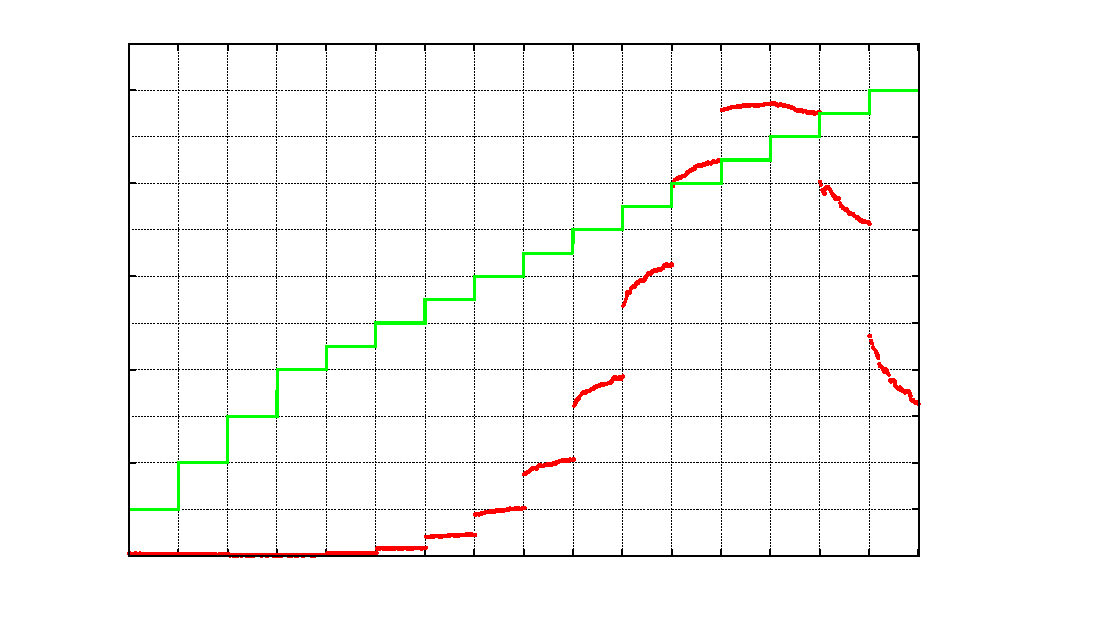
\includegraphics{1}}%
    \gplfronttext
  \end{picture}%
\endgroup

\caption{První měření (interval \SI{1}{\minute})}
\label{g:1}
\end{graph}

\begin{graph}[htbp] 
\centering
% GNUPLOT: LaTeX picture with Postscript
\begingroup
  \makeatletter
  \providecommand\color[2][]{%
    \GenericError{(gnuplot) \space\space\space\@spaces}{%
      Package color not loaded in conjunction with
      terminal option `colourtext'%
    }{See the gnuplot documentation for explanation.%
    }{Either use 'blacktext' in gnuplot or load the package
      color.sty in LaTeX.}%
    \renewcommand\color[2][]{}%
  }%
  \providecommand\includegraphics[2][]{%
    \GenericError{(gnuplot) \space\space\space\@spaces}{%
      Package graphicx or graphics not loaded%
    }{See the gnuplot documentation for explanation.%
    }{The gnuplot epslatex terminal needs graphicx.sty or graphics.sty.}%
    \renewcommand\includegraphics[2][]{}%
  }%
  \providecommand\rotatebox[2]{#2}%
  \@ifundefined{ifGPcolor}{%
    \newif\ifGPcolor
    \GPcolortrue
  }{}%
  \@ifundefined{ifGPblacktext}{%
    \newif\ifGPblacktext
    \GPblacktextfalse
  }{}%
  % define a \g@addto@macro without @ in the name:
  \let\gplgaddtomacro\g@addto@macro
  % define empty templates for all commands taking text:
  \gdef\gplbacktext{}%
  \gdef\gplfronttext{}%
  \makeatother
  \ifGPblacktext
    % no textcolor at all
    \def\colorrgb#1{}%
    \def\colorgray#1{}%
  \else
    % gray or color?
    \ifGPcolor
      \def\colorrgb#1{\color[rgb]{#1}}%
      \def\colorgray#1{\color[gray]{#1}}%
      \expandafter\def\csname LTw\endcsname{\color{white}}%
      \expandafter\def\csname LTb\endcsname{\color{black}}%
      \expandafter\def\csname LTa\endcsname{\color{black}}%
      \expandafter\def\csname LT0\endcsname{\color[rgb]{1,0,0}}%
      \expandafter\def\csname LT1\endcsname{\color[rgb]{0,1,0}}%
      \expandafter\def\csname LT2\endcsname{\color[rgb]{0,0,1}}%
      \expandafter\def\csname LT3\endcsname{\color[rgb]{1,0,1}}%
      \expandafter\def\csname LT4\endcsname{\color[rgb]{0,1,1}}%
      \expandafter\def\csname LT5\endcsname{\color[rgb]{1,1,0}}%
      \expandafter\def\csname LT6\endcsname{\color[rgb]{0,0,0}}%
      \expandafter\def\csname LT7\endcsname{\color[rgb]{1,0.3,0}}%
      \expandafter\def\csname LT8\endcsname{\color[rgb]{0.5,0.5,0.5}}%
    \else
      % gray
      \def\colorrgb#1{\color{black}}%
      \def\colorgray#1{\color[gray]{#1}}%
      \expandafter\def\csname LTw\endcsname{\color{white}}%
      \expandafter\def\csname LTb\endcsname{\color{black}}%
      \expandafter\def\csname LTa\endcsname{\color{black}}%
      \expandafter\def\csname LT0\endcsname{\color{black}}%
      \expandafter\def\csname LT1\endcsname{\color{black}}%
      \expandafter\def\csname LT2\endcsname{\color{black}}%
      \expandafter\def\csname LT3\endcsname{\color{black}}%
      \expandafter\def\csname LT4\endcsname{\color{black}}%
      \expandafter\def\csname LT5\endcsname{\color{black}}%
      \expandafter\def\csname LT6\endcsname{\color{black}}%
      \expandafter\def\csname LT7\endcsname{\color{black}}%
      \expandafter\def\csname LT8\endcsname{\color{black}}%
    \fi
  \fi
  \setlength{\unitlength}{0.0500bp}%
  \begin{picture}(10204.00,5668.00)%
    \gplgaddtomacro\gplbacktext{%
      \csname LT0\endcsname%
      \put(946,484){\makebox(0,0)[r]{\strut{} 0}}%
      \csname LT0\endcsname%
      \put(946,1378){\makebox(0,0)[r]{\strut{} 0.2}}%
      \csname LT0\endcsname%
      \put(946,2273){\makebox(0,0)[r]{\strut{} 0.4}}%
      \csname LT0\endcsname%
      \put(946,3167){\makebox(0,0)[r]{\strut{} 0.6}}%
      \csname LT0\endcsname%
      \put(946,4061){\makebox(0,0)[r]{\strut{} 0.8}}%
      \csname LT0\endcsname%
      \put(946,4956){\makebox(0,0)[r]{\strut{} 1}}%
      \csname LTb\endcsname%
      \put(1078,264){\makebox(0,0){\strut{}}}%
      \csname LTb\endcsname%
      \put(1524,264){\makebox(0,0){\strut{}}}%
      \csname LTb\endcsname%
      \put(1971,264){\makebox(0,0){\strut{}}}%
      \csname LTb\endcsname%
      \put(2417,264){\makebox(0,0){\strut{}}}%
      \csname LTb\endcsname%
      \put(2863,264){\makebox(0,0){\strut{}}}%
      \csname LTb\endcsname%
      \put(3310,264){\makebox(0,0){\strut{}}}%
      \csname LTb\endcsname%
      \put(3756,264){\makebox(0,0){\strut{}}}%
      \csname LTb\endcsname%
      \put(4202,264){\makebox(0,0){\strut{}}}%
      \csname LTb\endcsname%
      \put(4649,264){\makebox(0,0){\strut{}}}%
      \csname LTb\endcsname%
      \put(5095,264){\makebox(0,0){\strut{}}}%
      \csname LTb\endcsname%
      \put(5542,264){\makebox(0,0){\strut{}}}%
      \csname LTb\endcsname%
      \put(5988,264){\makebox(0,0){\strut{}}}%
      \csname LTb\endcsname%
      \put(6434,264){\makebox(0,0){\strut{}}}%
      \csname LTb\endcsname%
      \put(6881,264){\makebox(0,0){\strut{}}}%
      \csname LTb\endcsname%
      \put(7327,264){\makebox(0,0){\strut{}}}%
      \csname LTb\endcsname%
      \put(7773,264){\makebox(0,0){\strut{}}}%
      \csname LTb\endcsname%
      \put(8220,264){\makebox(0,0){\strut{}}}%
      \csname LTb\endcsname%
      \put(8666,264){\makebox(0,0){\strut{}}}%
      \csname LT1\endcsname%
      \put(8795,484){\makebox(0,0)[l]{\strut{} 0}}%
      \csname LT1\endcsname%
      \put(8795,931){\makebox(0,0)[l]{\strut{} 100}}%
      \csname LT1\endcsname%
      \put(8795,1378){\makebox(0,0)[l]{\strut{} 200}}%
      \csname LT1\endcsname%
      \put(8795,1826){\makebox(0,0)[l]{\strut{} 300}}%
      \csname LT1\endcsname%
      \put(8795,2273){\makebox(0,0)[l]{\strut{} 400}}%
      \csname LT1\endcsname%
      \put(8795,2720){\makebox(0,0)[l]{\strut{} 500}}%
      \csname LT1\endcsname%
      \put(8795,3167){\makebox(0,0)[l]{\strut{} 600}}%
      \csname LT1\endcsname%
      \put(8795,3614){\makebox(0,0)[l]{\strut{} 700}}%
      \csname LT1\endcsname%
      \put(8795,4061){\makebox(0,0)[l]{\strut{} 800}}%
      \csname LT1\endcsname%
      \put(8795,4509){\makebox(0,0)[l]{\strut{} 900}}%
      \csname LT1\endcsname%
      \put(8795,4956){\makebox(0,0)[l]{\strut{} 1000}}%
      \csname LT1\endcsname%
      \put(8795,5403){\makebox(0,0)[l]{\strut{} 1100}}%
      \csname LT0\endcsname%
      \put(176,2943){\rotatebox{-270}{\makebox(0,0){\strut{}$I/I_0$}}}%
      \csname LT1\endcsname%
      \put(9696,2943){\rotatebox{-270}{\makebox(0,0){\strut{}$U$ (\si{\volt})}}}%
      \csname LTb\endcsname%
      \put(4870,154){\makebox(0,0){\strut{}čas}}%
    }%
    \gplgaddtomacro\gplfronttext{%
    }%
    \gplbacktext
    \put(0,0){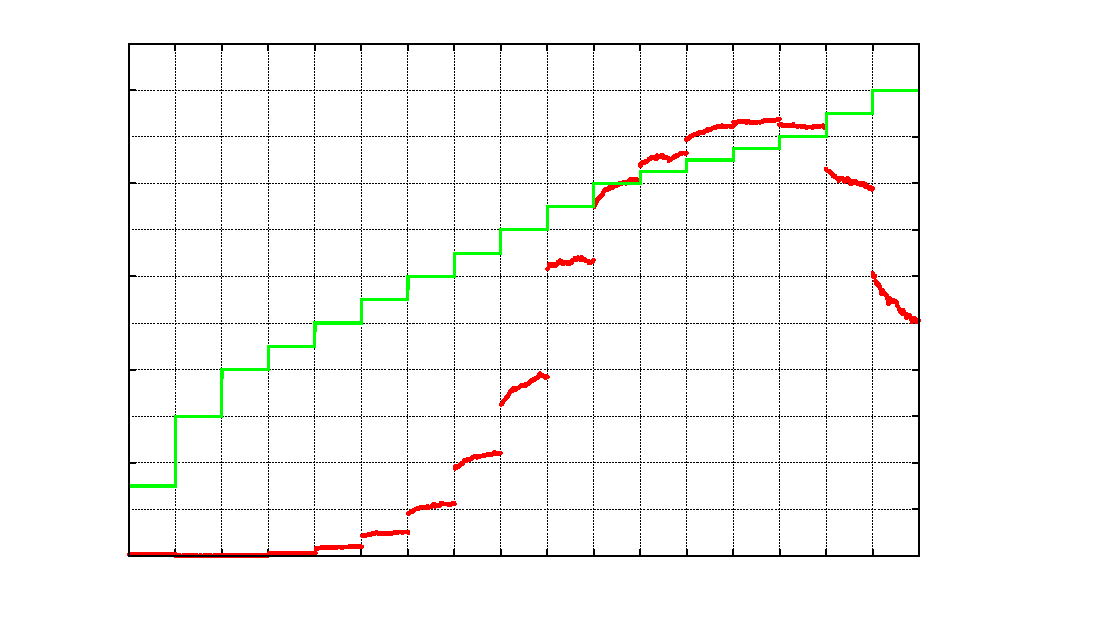
\includegraphics{2}}%
    \gplfronttext
  \end{picture}%
\endgroup

\caption{Druhé měření (interval \SI{2}{\minute})}
\label{g:2}
\end{graph}

Napětí na vzorku během měření kolísalo, maximální chybu odhadujeme na $\pm\SI{5}{\volt}$.

V obou případech jsme vzali poslední změřenou hodnotu (viz diskuze) a zanesli ji do tabulky \ref{t:1}.

\begin{tabulka}[htbp]
\centering
\begin{tabular}{cc|cc}
\multicolumn{2}{c|}{první měření} & \multicolumn{2}{c}{druhé měření} \\
$U$ (\si{\volt}) & $I/I_0$ & $U$ (\si{\volt}) & $I/I_0$ \\ \hline
100 & 0,004 & 150 & 0,003 \\ 
200 & 0,004 & 300 & 0,000 \\ 
300 & 0,002 & 400 & 0,002 \\ 
400 & 0,003 & 450 & 0,007 \\ 
450 & 0,006 & 500 & 0,021 \\ 
500 & 0,018 & 550 & 0,054 \\ 
550 & 0,045 & 600 & 0,119 \\ 
600 & 0,103 & 650 & 0,235 \\ 
650 & 0,207 & 700 & 0,410 \\ 
700 & 0,385 & 750 & 0,677 \\ 
750 & 0,625 & 800 & 0,860 \\ 
800 & 0,851 & 825 & 0,922 \\ 
850 & 0,970 & 850 & 0,983 \\ 
900 & 0,952 & 875 & 1,000 \\ 
950 & 0,713 & 900 & 0,982 \\ 
1000 & 0,327 & 950 & 0,841 \\ 
 &  & 1000 & 0,538 \\ 

\end{tabular}
\caption{Závislost intenzity na přiloženém napětí}
\label{t:1}
\end{tabulka}

\begin{graph}[htbp] 
\centering
% GNUPLOT: LaTeX picture with Postscript
\begingroup
  \makeatletter
  \providecommand\color[2][]{%
    \GenericError{(gnuplot) \space\space\space\@spaces}{%
      Package color not loaded in conjunction with
      terminal option `colourtext'%
    }{See the gnuplot documentation for explanation.%
    }{Either use 'blacktext' in gnuplot or load the package
      color.sty in LaTeX.}%
    \renewcommand\color[2][]{}%
  }%
  \providecommand\includegraphics[2][]{%
    \GenericError{(gnuplot) \space\space\space\@spaces}{%
      Package graphicx or graphics not loaded%
    }{See the gnuplot documentation for explanation.%
    }{The gnuplot epslatex terminal needs graphicx.sty or graphics.sty.}%
    \renewcommand\includegraphics[2][]{}%
  }%
  \providecommand\rotatebox[2]{#2}%
  \@ifundefined{ifGPcolor}{%
    \newif\ifGPcolor
    \GPcolorfalse
  }{}%
  \@ifundefined{ifGPblacktext}{%
    \newif\ifGPblacktext
    \GPblacktexttrue
  }{}%
  % define a \g@addto@macro without @ in the name:
  \let\gplgaddtomacro\g@addto@macro
  % define empty templates for all commands taking text:
  \gdef\gplbacktext{}%
  \gdef\gplfronttext{}%
  \makeatother
  \ifGPblacktext
    % no textcolor at all
    \def\colorrgb#1{}%
    \def\colorgray#1{}%
  \else
    % gray or color?
    \ifGPcolor
      \def\colorrgb#1{\color[rgb]{#1}}%
      \def\colorgray#1{\color[gray]{#1}}%
      \expandafter\def\csname LTw\endcsname{\color{white}}%
      \expandafter\def\csname LTb\endcsname{\color{black}}%
      \expandafter\def\csname LTa\endcsname{\color{black}}%
      \expandafter\def\csname LT0\endcsname{\color[rgb]{1,0,0}}%
      \expandafter\def\csname LT1\endcsname{\color[rgb]{0,1,0}}%
      \expandafter\def\csname LT2\endcsname{\color[rgb]{0,0,1}}%
      \expandafter\def\csname LT3\endcsname{\color[rgb]{1,0,1}}%
      \expandafter\def\csname LT4\endcsname{\color[rgb]{0,1,1}}%
      \expandafter\def\csname LT5\endcsname{\color[rgb]{1,1,0}}%
      \expandafter\def\csname LT6\endcsname{\color[rgb]{0,0,0}}%
      \expandafter\def\csname LT7\endcsname{\color[rgb]{1,0.3,0}}%
      \expandafter\def\csname LT8\endcsname{\color[rgb]{0.5,0.5,0.5}}%
    \else
      % gray
      \def\colorrgb#1{\color{black}}%
      \def\colorgray#1{\color[gray]{#1}}%
      \expandafter\def\csname LTw\endcsname{\color{white}}%
      \expandafter\def\csname LTb\endcsname{\color{black}}%
      \expandafter\def\csname LTa\endcsname{\color{black}}%
      \expandafter\def\csname LT0\endcsname{\color{black}}%
      \expandafter\def\csname LT1\endcsname{\color{black}}%
      \expandafter\def\csname LT2\endcsname{\color{black}}%
      \expandafter\def\csname LT3\endcsname{\color{black}}%
      \expandafter\def\csname LT4\endcsname{\color{black}}%
      \expandafter\def\csname LT5\endcsname{\color{black}}%
      \expandafter\def\csname LT6\endcsname{\color{black}}%
      \expandafter\def\csname LT7\endcsname{\color{black}}%
      \expandafter\def\csname LT8\endcsname{\color{black}}%
    \fi
  \fi
  \setlength{\unitlength}{0.0500bp}%
  \begin{picture}(10204.00,5668.00)%
    \gplgaddtomacro\gplbacktext{%
      \csname LTb\endcsname%
      \put(946,704){\makebox(0,0)[r]{\strut{} 0}}%
      \csname LTb\endcsname%
      \put(946,1558){\makebox(0,0)[r]{\strut{} 0.2}}%
      \csname LTb\endcsname%
      \put(946,2413){\makebox(0,0)[r]{\strut{} 0.4}}%
      \csname LTb\endcsname%
      \put(946,3267){\makebox(0,0)[r]{\strut{} 0.6}}%
      \csname LTb\endcsname%
      \put(946,4121){\makebox(0,0)[r]{\strut{} 0.8}}%
      \csname LTb\endcsname%
      \put(946,4976){\makebox(0,0)[r]{\strut{} 1}}%
      \csname LTb\endcsname%
      \put(1078,484){\makebox(0,0){\strut{} 0}}%
      \csname LTb\endcsname%
      \put(2665,484){\makebox(0,0){\strut{} 200}}%
      \csname LTb\endcsname%
      \put(4252,484){\makebox(0,0){\strut{} 400}}%
      \csname LTb\endcsname%
      \put(5839,484){\makebox(0,0){\strut{} 600}}%
      \csname LTb\endcsname%
      \put(7426,484){\makebox(0,0){\strut{} 800}}%
      \csname LTb\endcsname%
      \put(9013,484){\makebox(0,0){\strut{} 1000}}%
      \put(176,3053){\rotatebox{-270}{\makebox(0,0){\strut{}$I/I_0$}}}%
      \put(5442,154){\makebox(0,0){\strut{}$U$ (\si{\volt})}}%
    }%
    \gplgaddtomacro\gplfronttext{%
      \csname LTb\endcsname%
      \put(3322,5230){\makebox(0,0)[r]{\strut{}první měření}}%
      \csname LTb\endcsname%
      \put(3322,5010){\makebox(0,0)[r]{\strut{}druhé měření}}%
    }%
    \gplbacktext
    \put(0,0){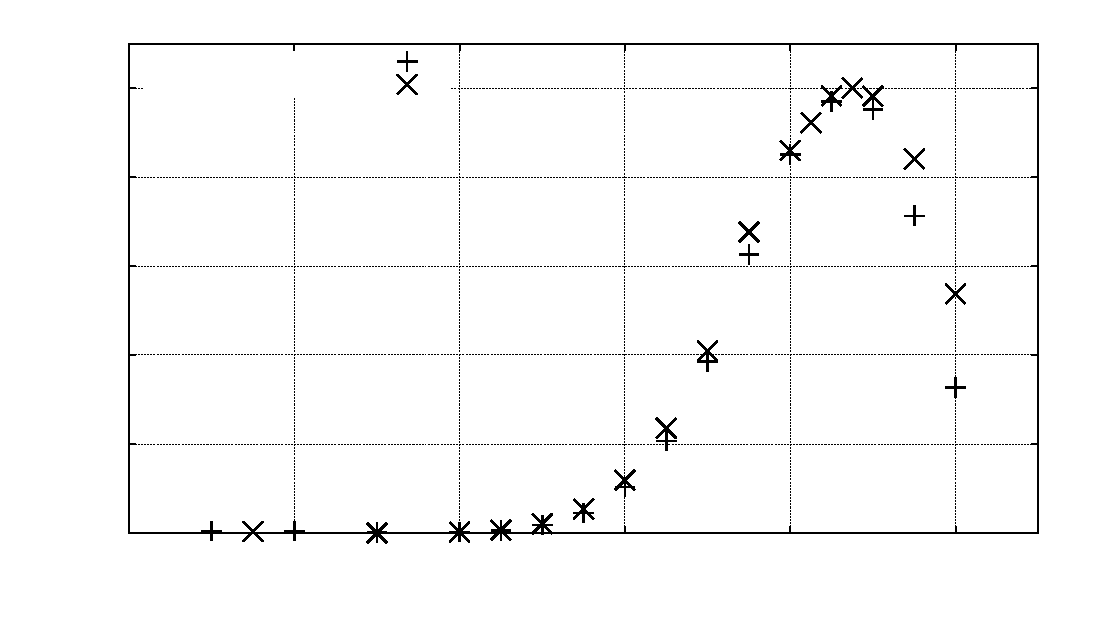
\includegraphics{3}}%
    \gplfronttext
  \end{picture}%
\endgroup

\caption{Závislost intenzity na přiloženém napětí}
\label{g:3}
\end{graph}

\begin{graph}[htbp] 
\centering
% GNUPLOT: LaTeX picture with Postscript
\begingroup
  \makeatletter
  \providecommand\color[2][]{%
    \GenericError{(gnuplot) \space\space\space\@spaces}{%
      Package color not loaded in conjunction with
      terminal option `colourtext'%
    }{See the gnuplot documentation for explanation.%
    }{Either use 'blacktext' in gnuplot or load the package
      color.sty in LaTeX.}%
    \renewcommand\color[2][]{}%
  }%
  \providecommand\includegraphics[2][]{%
    \GenericError{(gnuplot) \space\space\space\@spaces}{%
      Package graphicx or graphics not loaded%
    }{See the gnuplot documentation for explanation.%
    }{The gnuplot epslatex terminal needs graphicx.sty or graphics.sty.}%
    \renewcommand\includegraphics[2][]{}%
  }%
  \providecommand\rotatebox[2]{#2}%
  \@ifundefined{ifGPcolor}{%
    \newif\ifGPcolor
    \GPcolorfalse
  }{}%
  \@ifundefined{ifGPblacktext}{%
    \newif\ifGPblacktext
    \GPblacktexttrue
  }{}%
  % define a \g@addto@macro without @ in the name:
  \let\gplgaddtomacro\g@addto@macro
  % define empty templates for all commands taking text:
  \gdef\gplbacktext{}%
  \gdef\gplfronttext{}%
  \makeatother
  \ifGPblacktext
    % no textcolor at all
    \def\colorrgb#1{}%
    \def\colorgray#1{}%
  \else
    % gray or color?
    \ifGPcolor
      \def\colorrgb#1{\color[rgb]{#1}}%
      \def\colorgray#1{\color[gray]{#1}}%
      \expandafter\def\csname LTw\endcsname{\color{white}}%
      \expandafter\def\csname LTb\endcsname{\color{black}}%
      \expandafter\def\csname LTa\endcsname{\color{black}}%
      \expandafter\def\csname LT0\endcsname{\color[rgb]{1,0,0}}%
      \expandafter\def\csname LT1\endcsname{\color[rgb]{0,1,0}}%
      \expandafter\def\csname LT2\endcsname{\color[rgb]{0,0,1}}%
      \expandafter\def\csname LT3\endcsname{\color[rgb]{1,0,1}}%
      \expandafter\def\csname LT4\endcsname{\color[rgb]{0,1,1}}%
      \expandafter\def\csname LT5\endcsname{\color[rgb]{1,1,0}}%
      \expandafter\def\csname LT6\endcsname{\color[rgb]{0,0,0}}%
      \expandafter\def\csname LT7\endcsname{\color[rgb]{1,0.3,0}}%
      \expandafter\def\csname LT8\endcsname{\color[rgb]{0.5,0.5,0.5}}%
    \else
      % gray
      \def\colorrgb#1{\color{black}}%
      \def\colorgray#1{\color[gray]{#1}}%
      \expandafter\def\csname LTw\endcsname{\color{white}}%
      \expandafter\def\csname LTb\endcsname{\color{black}}%
      \expandafter\def\csname LTa\endcsname{\color{black}}%
      \expandafter\def\csname LT0\endcsname{\color{black}}%
      \expandafter\def\csname LT1\endcsname{\color{black}}%
      \expandafter\def\csname LT2\endcsname{\color{black}}%
      \expandafter\def\csname LT3\endcsname{\color{black}}%
      \expandafter\def\csname LT4\endcsname{\color{black}}%
      \expandafter\def\csname LT5\endcsname{\color{black}}%
      \expandafter\def\csname LT6\endcsname{\color{black}}%
      \expandafter\def\csname LT7\endcsname{\color{black}}%
      \expandafter\def\csname LT8\endcsname{\color{black}}%
    \fi
  \fi
  \setlength{\unitlength}{0.0500bp}%
  \begin{picture}(10204.00,5668.00)%
    \gplgaddtomacro\gplbacktext{%
      \csname LTb\endcsname%
      \put(946,704){\makebox(0,0)[r]{\strut{} 0}}%
      \csname LTb\endcsname%
      \put(946,1452){\makebox(0,0)[r]{\strut{} 0.5}}%
      \csname LTb\endcsname%
      \put(946,2200){\makebox(0,0)[r]{\strut{} 1}}%
      \csname LTb\endcsname%
      \put(946,2948){\makebox(0,0)[r]{\strut{} 1.5}}%
      \csname LTb\endcsname%
      \put(946,3695){\makebox(0,0)[r]{\strut{} 2}}%
      \csname LTb\endcsname%
      \put(946,4443){\makebox(0,0)[r]{\strut{} 2.5}}%
      \csname LTb\endcsname%
      \put(946,5191){\makebox(0,0)[r]{\strut{} 3}}%
      \csname LTb\endcsname%
      \put(2741,484){\makebox(0,0){\strut{}      200000}}%
      \csname LTb\endcsname%
      \put(4403,484){\makebox(0,0){\strut{}      400000}}%
      \csname LTb\endcsname%
      \put(6066,484){\makebox(0,0){\strut{}      600000}}%
      \csname LTb\endcsname%
      \put(7729,484){\makebox(0,0){\strut{}      800000}}%
      \csname LTb\endcsname%
      \put(9391,484){\makebox(0,0){\strut{}     1000000}}%
      \put(176,3053){\rotatebox{-270}{\makebox(0,0){\strut{}$\arcsin \sqrt{I/I_0}$}}}%
      \put(5442,154){\makebox(0,0){\strut{}$U^2$ (\si{\volt\squared})}}%
      \put(4445,3247){\makebox(0,0)[l]{\strut{}$y=\num{2.97e-6}\cdot x-\num{0.716}$}}%
    }%
    \gplgaddtomacro\gplfronttext{%
      \csname LTb\endcsname%
      \put(3322,5230){\makebox(0,0)[r]{\strut{}první měření}}%
      \csname LTb\endcsname%
      \put(3322,5010){\makebox(0,0)[r]{\strut{}druhé měření}}%
      \csname LTb\endcsname%
      \put(3322,4790){\makebox(0,0)[r]{\strut{}fit}}%
    }%
    \gplbacktext
    \put(0,0){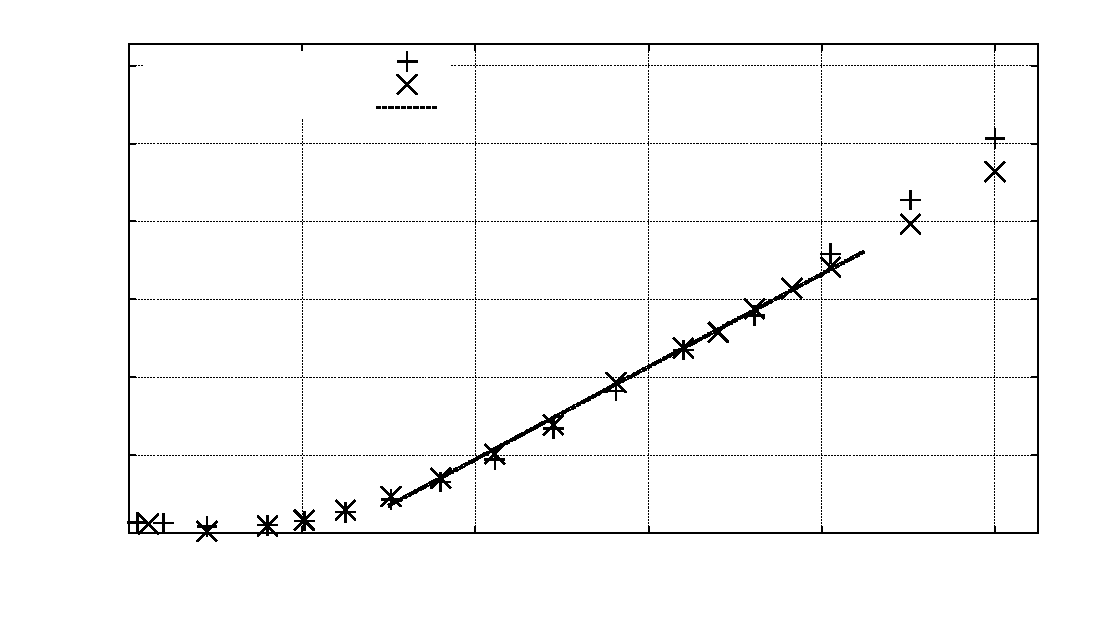
\includegraphics{4}}%
    \gplfronttext
  \end{picture}%
\endgroup

\caption{K určení Kerrovy konstanty}
\label{g:4}
\end{graph}

Z tabulky \ref{t:1} jsme určili z druhého měření půlvlnné napětí
\begin{equation*}
U_p=\SI{875(20)}{\volt} \,,
\end{equation*}
v prvním měření byl výsledek stejný, jen méně přesný.

V programu gnuplot jsme lineární regresí závislosti \eqref{e:fit} určilli konstantu úměrnosti (viz graf \ref{g:4})
\begin{equation*}
K \frac{\pi l}{d^2} = (\num{2.97(6)})\SI{e-6}{\per\volt\squared}
\end{equation*}
a dostáváme Kerrovu konstantu
\begin{equation*}
K = (\num{1.24(4)})\SI{e-6}{\metre\per\volt\squared} \,.
\end{equation*}
Hodnota získaná z prvního měření by se zřejmě příliš nelišila (viz graf \ref{g:4}).

%Diskuze výsledků
\section*{Diskuze}
Z grafů \ref{g:1} a \ref{g:2} je vidět, že vzorek reaguje na změny elektrického pole velmi pomalu. Je možné také usuzovat, že čím silnější pole je, tím pomaleji na něj vzorek reaguje (např. při změny z 950 na \SI{1000}{\volt} intenzita i po dvou minutách velmi rychle klesá, u nižších napětí tento jev není tak výrazný). 

V prvním i druhém měření vyšla téměř totožná závislost (viz graf \ref{g:3}). Hodnoty se mírně liší, ale pro naše účely by stačilo měřit s intervalem \SI{1}{\minute}.

V grafu \ref{g:4} ve skutečnosti není na svislou osu vynesen $\arcsin$. V rozsahu, ve kterém se pohybujeme, není $\sin^2$ prostá funkce, proto jsme pro napětí větší než půlvlnné vynesli funkci $\pi-\arcsin$.

Během celého průběhu druhého měření nevystoupala intenzita na vyšší hodnotu než \SI{94}{\percent} $I_0$. To by se~v našem uspořádání nemělo stát, obvzláště podezřelé je, že na druhé měření $I_0$ vzrostla, ale hodnoty $I$ měly maximum přibližně stále stejně jako v prvním měření. Usoudili jsme tedy, že naměřená $I_0$ je chybná a nahradili ji maximem za celé měření.

Hodnoty v tabulce \ref{t:1} jsme vzali jako poslední naměřené hodnoty v grafech \ref{g:1} a \ref{g:2}. To by mělo dobrý smysl, kdyby už byla intenzita ustálená, tedy pro napětí do \SI{900}{\volt} tyto hodnoty považujeme za správné. Nicméně z~grafů je zřejmé, že pro vyšší napětí intenzita jistě ustálená ještě není, a proto je zatížena velkou chybou.
Z~tohoto důvodu jsme také tyto body vyřadili z fitu.

Přestože v rovnici \eqref{e:fit} žádný absolutní člen nefiguruje, při lineární regresi jsme ho použili. Důvodem je, že závislost žádné přímce procházející počátkem dobře neodpovídá (pokud nechceme fitovat pouze první čtyři téměř nulové hodnoty). Vybrali jsme tedy větší část rozsahu, která se chová afinně, a tu nafitovali. Příčinou této nepříjemnosti možná mohla být např. nelinearita vzorku nebo špatně zkřížené polarizátory.

Při výpočtu Kerrovy konstanty jsme používali parametry $l$ a $d$, o kterých předpokládáme, že jejich chyba je zanedbatelně malá. Pokud by tomu tak nebylo, mohly ovlivnit správnost našeho výsledku.

%Závěr
\section*{Závěr}


\printbibliography[title={Seznam použité literatury}]

\end{document}